% https://www.overleaf.com/read/jydxqkkkskzp
% https://github.com/MCG-NKU/NSFC-LaTex
% by Ming-Ming Cheng https://mmcheng.net

\documentclass[12pt]{article}
\usepackage[UTF8]{ctex}
\usepackage{nsfc}
\usepackage{url}
\def\UrlBreaks{\do\A\do\B\do\C\do\D\do\E\do\F\do\G\do\H\do\I\do\J
\do\K\do\L\do\M\do\N\do\O\do\P\do\Q\do\R\do\S\do\T\do\U\do\V
\do\W\do\X\do\Y\do\Z\do\[\do\\\do\]\do\^\do\_\do\`\do\a\do\b
\do\c\do\d\do\e\do\f\do\g\do\h\do\i\do\j\do\k\do\l\do\m\do\n
\do\o\do\p\do\q\do\r\do\s\do\t\do\u\do\v\do\w\do\x\do\y\do\z
\do\.\do\@\do\\\do\/\do\!\do\_\do\|\do\;\do\>\do\]\do\)\do\,
\do\?\do\'\do+\do\=\do\#} 


\newcommand{\note}[1]{\textcolor[rgb]{0.6,0,0}{note: #1}}
\newcommand{\todo}[1]{{\textcolor{red}{\bf [#1]}}}
\newcommand{\myPara}[1]{\paragraph{#1:}}

\graphicspath{{figures/}}


\begin{document}



%%%%%%%%% TITLE

\title{报告正文}
% title: 危化品智能装配中的高精度6D姿态估计方法研究
\maketitle
\thispagestyle{empty}

\ContentDes{(一)立项依据与研究内容(建议8000字以下):}


\NsfcSection{1}{项目的立项依据}{
(研究意义、国内外研究现状及发展动态分析,需结合科学研究发展趋势来论述科学意义;或结合国民经济和社会发展中迫切需要解决的关键科技问题来论述其应用前景。附主要参考文献目录);}

\subsection{研究意义}

爆炸品、有毒化工、放射性物质、生物化学制剂等危化品的装配工艺,对于制备环境要求很苛刻。工厂装配过程中,为了确保装配安全性,对产线工人的年龄、工作时间和操作流程等都有严格的要求。以工程炸药制备公司为例,为了保障安全生产,工人正常上工前需培训6个月,每天工作时间不能超过6小时,每项工艺流程需双人确认。这些安全措施极大限制了工厂的产能,需要通过智能制造技术替代人工,提升产能。

% 此处表述6D姿态估计是智能装配中的关键技术,为了提升精度,需要用多传感器融合
待装配物件的六自由度(6D)姿态估计是智能装配的关键技术,其核心问题是高精度的姿态估计。与普通的工业自动化设备不同,危化品的装配操作流程裕度很小,无法通过降低机械操控设备的控制精度和重访精度实现无人操作。智能装配工艺通过装置在产线上的传感器,估计炸药、放射性元素、腐蚀性药品等空腔的姿态,在操控链路形成负反馈,精准完成原料装填和定位螺丝的紧固。

% 传统的6D姿态估计采用RGB或RGBD的方式计算姿态,准确度以目标物体点云的10%作为度量,无法满足精准装配的需要,亟需改进;当前的学术研究中,6D姿态估计算法估计的准确度以目标物体点云尺度的10\%作为度量,其精度只适用于普通物件如快递包裹、日常物品等的粗抓取,无法满足危化品装配的精细操控要求。
面向危化品智能装配的6D姿态估计需要解决三个核心问题,其一为弱纹理表面的算法适应性问题,其二为有遮挡情况下的鲁棒估计问题,其三为姿态估计的高精度修正问题。本项目融合可见光、深度图和光谱相机的影像特征,通过分析多模态传感器数据的特征表达,提取和对齐不同模态的特征,并通过交叉验证抑制单一模态中的噪声,融合有效的互补信息,提升6D姿态估计的适应性、鲁棒性和精度,解决危化品智能装配中的高精度姿态估计难题。

\subsection{国内外相关工作}

大多数姿态估计方法遵循两阶段的范式,首先检测图像中的目标物体,之后在缩放后的目标物体区域上进行姿态估计。尽管现有方法在大多数简单的场景下表现良好,但由于所使用的检测器对弱纹理或被遮挡工件的检测效果并不理想,算法在智能装配应用中的性能急剧下降。

对于第一阶段的目标检测任务,常用的检测方法有两段式和单段式两类\cite{ATSS, fcosv1, fcosv2, PAA, faster-rcnn, maskrcnn}。两段式检测方法首先采用区域建议网络~\cite{faster-rcnn, maskrcnn}生成边界框候选体,然后由分类和细化网络处理,去除假阳性,并调整边界框的位置和大小。这种策略准确度较高,但成本高,效率低。单段式检测器通过在编码器的最终特征图中的每个空间位置用一组预定义的锚框代替区域建议网络来解决这个问题~\cite{fcosv1,retinanet,yolov1}。这种方法会导致锚点中存在大量负样本,虽然这一问题可以通过focal loss~\cite{retinanet,fpn}在一定程度上解决,但程度有限,早期的单段式检测器并没有达到两段式检测器的精度。Zhang~\cite{ATSS}通过一个简单而有效的正样本策略解决了这一问题。最近的大多数检测方法都遵循类似的策略~\cite{fcosv2, PAA, autoassign, OTA, TTF, yolov3},相关改进算法的准确性比两段式方法更好,同时效率更高。但即便如此,这些方法都假设场景中物体的纹理相对丰富,且具有较少的遮挡,与智能装配的6D物体姿态估计场景中的特性仍有较大差异。

% 弱纹理物体位姿估计解决方案:在数据输入源头上解决,即增加depth图像和高光谱图像,实现多源融合。
危化品工件的表面大多没有纹理,这种工况下的目标检测是姿态估计中的一个难点。仅通过RGB图像估计的位姿精度不高,鲁棒性较差。一方面,深度学习网络很难从单幅RGB图像中提取有效的颜色和几何特征,另一方面,三维物体到二维像平面的投影过程丢失了三维结构的几何约束,单幅图像无法逆推结构信息。
基于RGB-D的6D位姿估计方法可以利用点云的三维几何特征来预测目标姿态,其估计精度比单幅RGB图像更高。这类算法的难点在于RGB图和深度图两种异构数据的融和。目前解决的思路有三类。
第一类为像素级融合方法,先利用2D检测或分割网络提取RGB图像特征,将图像特征传递给深度图生成的点云,然后将增强后的点云反馈给点云3D目标检测器。2D检测的结果可辅助三维点云形成3D视锥\cite{Qi2018},减小候选区域的范围。所形成的的视锥也可以进一步划分为网格单元\cite{Wang2019}进行3D检测。或者2D分割的结果也可用于增强3D点云\cite{Vora2020},将增强后的点云输入3D目标检测器提升检测效果。这类方法以顺序的方式进行融合,效率相对较低。
第二类为特征级融合方法,在基于点云的3D目标检测器的中间阶段融合图像和点云特征。例如,在基于网格的检测网络骨干的中间层中使用连续卷积\cite{Liang2018, Liang2019}、混合体素特征编码\cite{Sindagi2019}或Transformer\cite{Zhang2022}网络等融合算子进行多模态融合。
第三类为决策级融合,将RGB图像和Depth图像生成的点云数据通过两个独立网络分别生成2D和3D检测框\cite{Asvadi2018}并融合输出。这种方法可以更好地借鉴每个独立任务的SOTA算法,避免中间特征层上的信息交互,执行效率高,但无法利用不同模式的互补语义信息\cite{Pang2020}提升检测精度。

%本项目在特征级融合的基础上,引入UV数据保持深度图点特征三维空间位置的一致性,从而在异构输入源之间解决视角对齐的问题。
与普通工业零件不同,危化品工件中通常有危险度较高的化学部件,如易爆、有毒或有辐射的填充物。对于这类区域的精细检测和分割,一方面可以避免误操作减少事故,另一方面可为检测网络提供更精准的边界区域特征。不同的化学元素在特定的光谱谱段有脉冲响应特性,可通过光谱相机清晰地定位物质边界,能显著提升姿态估计第一阶段的检测和分割精度。光谱图像的检测和分割算法思路与可见光图像相似,最主要的问题在于样本数据较少,且分布不均匀,业界没有大规模数据集可用于网络训练。目前解决这一问题的主要方法是小样本学习\cite{lys2022targetDetection, shi2020HyperspectralTargetDetection}或加强注意力机制\cite{shi2020hyperspectralROI}。

% 此处描述 RGB, Depth, 和光谱数据融合的国内外现状
对于同一场景下的可见光、深度图和光谱图像的融合处理,目前没有可直接借鉴的方法,但多传感器融合的方法在遥感影像处理和自动驾驶领域\cite{feng2021}中都有相关研究。一种朴素的融合方法是决策级融合,对不同的输入数据分别提取特征图\cite{pang2020clocs},构建基于统计的特征加权组合模块,对不同输入分支提取的特征赋予不同的权重,在输出层进行决策级融合\cite{li2022sal}。这种方法既可以区分不同输入源特征在分类器中的重要性,又可以避免特征提取网络学习本身对分类结果的干扰。但它没有考虑多源数据特征间的差异性与互补性。另一种思路是特征级融合,先前的研究有两种模式,其中一种模式以Xie等人提出的Pi-rcnn\cite{xie2020pircnn}和Vora等人提出的Pointpainting\cite{vora2020pointpainting}为代表,将三维点云中的每一个点投影到二维像平面,然后通过双线性插值获得对应二维图像特征。这种方式虽然在像素级进行了细粒度的特征聚合,但是该操作过程由于融合点的稀疏性而失去二维图像密集特征的优势,即破坏了二维图像特征的语义一致性。另一种方式以Chen等人提出的MV3D\cite{chen2017multi}为代表,利用3D目标检测器分别获取点云数据和二维RGB图像中初始建议框,然后融合两种模态感兴趣区域特征。这种方式通过实例级融合保持了语义的一致性,但是利用3D目标检测器获取初始建议框的阶段所提取的特征相对粗糙,且缺失二维图像中的稠密信息表征。

% 在对不同输入源的数据进行特征抽取时,增加三维交叉注意力模块\cite{li2022triplet}增强多源数据的互补空间特征,并进行逐层特征融合。这种方法在自动驾驶领域\cite{huang2020epnet}取得了不错的结果。\note{补充特征级融合的问题}先前的研究有两种模式:一是将三维点云中的每一个点投影到二维的像平面,然后通过双线性插值获得对应的二维图像特征。这种方式虽然在像素级进行了细粒度的特征聚合,但是该操作过程由于融合点的稀疏性而失去光谱图像密集特征的优势,即破坏了二维光谱图像特征的语义一致性。另一种方式是利用3D目标检测器分别获取点云数据和光谱图像中初始建议框,然后融合两种模态感兴趣区域特征。这种方式通过实例级融合保持了语义的一致性,但是利用3D目标检测器获取初始建议框的阶段提取的特征相对粗糙且缺失光谱图像中的稠密信息表征。


% 有遮挡情况下的鲁棒估计现状
遮挡是6D姿态估计中的另一个难点问题,通用的目标检测方法假设物体之间遮挡较少,标准真值包围框中心的区域周围为目标物体,因此在网络学习中专注于仅从这些区域提取的样本预测边界框参数。然而,在有遮挡的情况下,真值包围框的中心通常被其他物体或者场景元素遮蔽,导致检测框出现较大偏差。为了提升姿态估计的性能,大多数方法需要依赖额外的姿态修正组件。这些组件首先根据初始姿态以及物体的CAD模型渲染合成图像,然后基于光流网络估计渲染图像和输入目标图像之间的密集2D-to-2D对应关系。在利用目标的3D形状信息将2D对应关系提升到3D-to-2D对应关系之后,基于PnP算法迭代计算更精细的姿态参数。

这种算法框架在大多数通用场景下表现良好,但它有几个缺点。
首先,所使用的光流网络建立在两个假设之上,即两个潜在匹配之间的亮度一致性和本地邻居内匹配的平滑度。这一假设在通用场景下是成立的,但在智能装配的6D物体姿态估计场景下,我们没有关于目标形状的线索,缺少形状约束,从而导致目标图像中每个像素的潜在匹配空间盲目扩大。
其次,匹配过程中物体形状信息的缺失会导致匹配结果出现明显偏差,在PnP姿态求解过程中引入显著噪声。
另外,在这种两阶段的框架中,第一阶段的训练依赖于匹配网络的损失函数,该匹配损失不能直接反映最终的6D姿态估计损失,且不是端到端可训练的。

近几年的位姿估计方法,通过使网络预测一些预定义的3D关键点~\cite{rad2017bb8, hu2019segDriven, peng2019pvnet, Hu2021},或对每个2D像素预测稠密的对应3D点~\cite{zakharov2019dpod, Su2022, li2019cdpn, wang2021gdrnet, Di2021}来创建对应关系。之后通过数值PnP求解器~\cite{lepetit2009epnp}或直接从中间对应关系的表达来学习姿态~\cite{hu2020singleStage, EroPnP,wang2021gdrnet, Di2021}。通过精心设计卷积神经网络结构改进的算法~\cite{he2016resnet, resnext_2017_cvpr}在鲁棒性和准确性方面都有显著提升~\cite{Xiang2018, peng2019pvnet, wang2019densefusion60},但复杂的杂乱场景下,姿态估计的准确性依然不高。

对于6D姿态的修正,以往的方法主要依赖于已配准的深度图~\cite{Xiang2018, li2019cdpn, wang2019densefusion60},但在许多真实场景~\cite{Hu2021}中深度图难以直接获取。
近几年的姿态修正方法使用无需深度数据的“渲染-比较”策略,可以获得性能相当或更好的结果~\cite{li2018deepim, zakharov2019dpod, cosypose, rad2017bb8, Hu2022, Lipson2022, RNNPose_2022_cvpr,Repose_2021_iccv}。Hu等~\cite{Hu2022}近期提出的6D姿态修正方法与这一策略有所不同,他将6D姿态修正问题建模为渲染图像到目标图像之间的2D匹配关系问题,通过数值求解获得修正之后的姿态。算法精度比“渲染-比较”的策略更高,但由于该方法将6D姿态修正建模为无约束的纯2D到2D匹配问题,脱离了6D物体姿态的物理意义,因此理论上讲估计结果是次优的。为了提升性能,申请人团队提出了一个由目标的3D形状引导的形状约束递归匹配框架,在精度和效率方面都有了大幅提升。

% 为了解决当前检测器在遮挡环境下的退化问题,我们提出了一种检测方法,该方法利用了6D姿态估计中目标对象是刚性的这一特性。
% 对于此类对象,任何可见部分都可以提供完整边界框的可靠估计。因此,我们认为,与标准物体检测器使用的基于中心的采样相比,任何从可见部分提取的特征都应该是训练期间正样本的潜在候选。
对于危化品智能装配中的三个核心问题,每个细分学术领域的学者及申请人团队都有相关的基础研究。在多模融合解决弱纹理物体的检测方面,可见光和深度图像融合估计已有可借鉴的算法框架,但如何有效融合光谱数据仍需探索。有遮挡下的鲁棒估计是目前6D姿态估计中的一个公认难题,通过改进网络结构和融合策略提升鲁棒性目前算法改进的主要思路。而对于高精度姿态修正问题,基于几何引导的约束框架是目前探索的行之有效的解决方案,但仍有很大的改进空间。

{
\bibliographystyle{IEEEtran}
\bibliography{nsfc_sr}
}


%%%%%%%%%%%%%%%%%%%%%%%%%%%%%%%%%%%%%%%%%%%%%%%%%
\NsfcSection{2}{项目的研究内容、研究目标,以及拟解决的关键科学问题}{
(此部分为重点阐述内容);}

\subsection{研究目标}

针对危化品智能装配中6D位姿估计中的工件表面弱纹理、工件叠放有遮挡和位姿估计精度不满足自动化操控需求这三个核心问题,研究融合可见光、深度图和光谱图的检测和姿态估计深度学习网络,分析智能装配场景下影响目标检测准确度和姿态估计精度的因素,从网络结构、损失函数和融合策略等方面改进算法,提升工件姿态估计的精度,满足危化品智能装配对工件姿态估计精度的要求。预期发表学术研究论文10篇,其中顶会或顶刊论文8篇,申请专利和软件著作权8件。

\subsection{研究内容}

% 0. 总述
分析可见光、深度图和光谱相机数据的匹配关系,研究互补融合表征的方法,解决工件表面弱纹理情况下的目标检测问题;研究刚性物体的感知检测网络结构,提升有遮挡情况下的目标检测精度;改进基于CAD模型几何特征引导的姿态修正模块,提升姿态修正的准确度。对三个分支的改进策略在不同网络层级进行融合,研究高效复合的深度学习网络,提升工件6D姿态估计的精度。主要研究内容包括以下三部分:
% --- 参考
% 为了解决同类研究在真实复杂环境下暴露的不足,本课题组研究涉及危险设备智能装配环境下基于几何特征引导的目标六自由度姿态估计问题,并融入多源融合表征以及多模态3D目标检测框架。研究内容可提炼为三个方面,它们互相联系构成完整的面向危险设备智能装配零部件的六自由度姿态估计系统。

% 1. 可见光、深度图和光谱图的特征融合方法
1. 面向弱纹理工件的目标检测任务,研究多模态影像数据的融合表征方法。研究不同模态数据特征的提取和对齐方法,分析在不同空间尺度和特征层深度进行信息交叉对弱纹理工件检测结果的影响,以及主从式融合网络结构对位姿估计结果的影响,通过原理分析和实验验证探索危化品装配中对弱纹理工件检测任务的最佳多模融合方法。

% 删除了对等网络

% --- 参考
%\textbf{A、面向危险设备智能装配零部件的多源融合表征}
%针对危险设备智能装配零部件的多源融合表征多模态对齐融合的问题和挑战,以融合方案对位姿估计优化后的精度为评价依据,研究多模态信息的表达和特征提取。研究该过程包含两个细节问题:(1)针对目标数据的差异性以及不同模态数据对于姿态估计任务的重要性,解决姿态估计问题中多种信息表达的关键问题,制定高效针对性的目标特征提取策略;(2)研究神经网络下多模态特征的信息对齐和融合问题,提出可行的多模态信息融合方式。


% 2. 有遮挡情况下的目标检测精度
2. 有遮挡情况下的刚性工件目标检测精度提升方法。研究如何利用目标边界框中的所有3D空间信息指导生成可见性掩膜,避免场景元素遮挡下掩膜不可用的问题。研究如何使用可见性掩膜指导网络训练时对候选目标的抽样,同时研究如何充分利用刚体的局部特征获得的先验知识,使网络的训练和推理过程由刚体可见部分监督和融合,避免遮挡部分的干扰。分析通道融合策略,通过融合多个可靠局部区域的预测结果,提升工件整体检测的准确度。

% --- 参考
%\textbf{B、针对危险设备智能装配零部件复杂环境下的3D目标检测}
%主流的目标检测算法在通用数据集上可以实现高精度、高实时性的目标检测。这类方法通常使用特征金字塔网络(FPN)来输出比例丰富的特征图,然后将每个特征向量作为训练样本,由分类分支和回归分支进行进一步处理。这类框架成功的关键在于训练期间选择正样本并且假定真实边界框中心的区域能够提供目标信息,即不被其它物体遮挡。然而在工业零的部件所处的复杂环境中,目标经常受到严重遮挡,无法满足中心假设。另外,常规的目标检测算法没有考虑使用刚性目标的可见部分为边界框的预测提供信息。针对以上问题和挑战,本课题将研究一种刚性感知检测方法来提高目标检测精度。具体包含三个以下问题:第一,如何利用目标边界框中的所有像素信息来指导生成可见性掩膜,避免场景元素遮挡下的掩膜不可用的问题;第二,如何使用可见性掩膜指导训练期间对候选目标的抽样,使得网络由所有可见部分监督并且丢弃遮挡部分;第三,如何融合所有高可靠性候选局部预测,以产生更加鲁棒的检测结果。0



% 3. 基于几何引导的姿态修正
3. 基于工件几何特征引导的位姿修正方法。基于CAD模型将工件的几何特征在每一次迭代的位姿下进行投影,分析和设计有效的网络结构和特征嵌入策略,将几何信息引入目标图像与渲染图像的特征匹配过程,对6D姿态表达方式以及误差损失函数进行精细化设计,提升每次迭代的度量精度。


% --- 参考
%\textbf{C、面向工业机械臂抓取基于零部件CAD模型几何特征引导的目标六自由度姿态估计网络设计}
%基于检测-估计-修正的6D姿态估计框架显示出了优良的性能,被近期提出的大多数方法所采用。采用一个单独的6D姿态修正网络可以放松对前一级估计网络的要求。同时基于CNN的6D姿态修正网络的输入为目标图像与在前一级估计网络得到的粗糙姿态下的渲染图像,这样的输入可以减轻姿态修正网络对数据的需求。目前大多数方法通过估计目标图像与渲染图像之间的对应关系来求解目标图像中物体的6D姿态。然而这种方法很强地依赖于物体的纹理特征,而对于工业零部件,大部分物体呈现出弱纹理或者弱纹理的特征,因此这种方法应用于工业零部件上会有很强的局限性。因此对于弱纹理或者弱纹理的工业零部件,物体的几何特征需要被有效地利用,然而现有的姿态修正方法很少探索物体的几何特征。
%本课题拟提出一个基于物体几何特征的6D姿态修正方法。在现有的基于纹理特征的对应关系估计网络中,如RAFT,本文通过利用点云特征提取网络,显式地将物体的几何特征进行编码,作为对应关系估计网络的参考信息。在迭代优化过程中,对应关系估计网络全局地通过可微姿态求解层来修正在上一步迭代过程中求解得到的姿态。具体来说,将物体的几何特征在上一步估计得到的姿态下进行投影,同时将物体的几何信息引入目标图像与渲染图像的特征匹配过程中,结合特征匹配结果与投影得到的几何特征来全局地求解更新之后的目标物体的6D姿态。



\subsection{拟解决的关键科学问题}

本课题拟解决以下三个关键科学问题:

1. 弱纹理工件的可见光、深度图和光谱图的有效融合表征问题。在弱纹理条件下,光谱数据可捕获准确的材质信息,为基于可见光图像和深度图的区域分割提供稀疏但可靠的先验。如何充分挖掘深度图和光谱数据对可见光图像特征提取的引导和补偿,实现多模态数据在姿态估计任务中的协同表达是本课题需要解决的关键科学问题。

2. 有遮挡情况下的工件3D目标检测鲁棒性问题。智能装配场景中工件存在相互遮挡的情况,基于目标中心区域抽样进行估计的方法不再适用。尽管理论上可以将该问题进行拆分,建模为目标分割任务,通过标注以及目标物体掩膜估计来区分目标前景以及背景,但像素级的掩膜标记成本过高。本课题研究的装配流程中的危化品通常为刚体,这常规目标检测任务有所不同,如何利用这一特性降低掩膜标注的要求,提高检测鲁棒性,是3D目标检测中的关键问题。

3. 位姿修正中的工件CAD模型几何特征引导问题。当前算法中6D姿态修正都依赖物体表面的纹理,对于弱纹理工件,这一方法不再适用。现有姿态修正方法中,将3D问题通过渲染技术转换成无约束的2D匹配问题,搜索空间巨大,严重制约匹配的精度和效率。如何在位姿修正的2D匹配中引入3D几何约束,提高姿态修正精度,是本课题要解决的关键问题。



\NsfcSection{3}{拟采取的研究方案及可行性分析}{
(包括研究方法、技术路线、实验手段、关键技术等说明);}

\iffalse
\subsection{拟采取的技术路线}
\fi

\begin{figure}[h]
	\centering
    \begin{overpic}[width=0.85\columnwidth]{multi_model_sensors.jpg}
    \end{overpic}
    \caption{危化品装配场景及多模传感器影像示意图,其中(a)为智能装配场景示意图,本课题研究的实际场景中工件无法固定,且有多个不同模态的相机;(b)为可见光图像,工件和场景的纹理和色彩较为丰富;(c)为深度图,反映场景中物体离相机的距离;(d)为光谱图,在感兴趣材质对应的谱段有单峰响应;
    }\label{fig:scene_demo}
\end{figure}

危化品智能装配的工作场景示意图如\ref{fig:scene_demo}所示。实际工作场景中,危化品部件只能通过机械导流摆正,但无法紧固,需要智能抓取。实际环境中装置了可见光相机、深度相机和光谱相机,对同一场景进行拍摄。可见光图像中工件和场景的纹理和色彩较为丰富,能够提取的特征维度多,但每一维度特征的显著性不强。深度图只反映场景中物体离相机的距离。在选定光谱谱段后,光谱相机输出的图像中感兴趣物体材质区域的光谱有单峰响应,其他区域的响应图较弱,如图(d)所示。在本课题的多模数据融合姿态估计方案中,数据之间的配准很关键,但不属于本课题的研究范围。本课题的输入数据为已配准好的可见光、深度图和光谱图像。

\begin{figure}[h]
    \centering
    \begin{overpic}[width=\columnwidth]{solution.jpg}
    \end{overpic}
    \caption{课题研究整体方案及内容安排}
    \label{fig:research_solution}
\end{figure}

本课题的整体研究框架如图\ref{fig:research_solution}所示。前期我们将着重方法研究,在现有的T-LESS\cite{tless2017}和ITODD\cite{itodd2017} 等RGB-D 6D姿态数据集上通过手工标记增加目标物体的光谱响应图,生成用于算法思路验证的多模态数据集。T-LESS和ITODD数据集包含目标场景的可见光图像和深度图,目标检测和分割的真值,以及6D姿态估计的真值,手工标记光谱响应图之后,可用于支撑本课题的前期算法验证。本课题的研究内容之间有相对顺序的关系,在后续阶段算法未改进时,将用现有的SOTA方法完成整体算法流程的计算。算法在模拟数据集上完成验证后,我们将在真实装配场景中验证算法的精度,并迭代更新。
\begin{figure}[h]
    \centering
    \begin{overpic}[width=0.9\columnwidth]{top_arch.JPG}
    \end{overpic}
    \caption{算法研究总体框架}
    \label{fig:top_arch}
\end{figure}
课题主要包含三部分研究内容,分别为多源融合表征网络研究、复杂环境下的3D目标检测网络研究和基于CAD模型几何特征引导的姿态修正网络研究。每一部分着重研究精度提升中的一个关键环节,三部分之间的关系如图\ref{fig:top_arch}所示。对多源融合表征网络的研究部分,我们将探究不同阶段、模式和组合的融合对于可见光、深度图和光谱图特征的有效表征能力,网络输出融合特征和目标位置的掩膜。研究初期我们用SOTA的目标检测和姿态修正算法验证特征表征的有效性。对于3D目标检测网络部分,有遮挡情况下的关键点检测和融合是算法研究的关键,我们将注重研究有遮挡条件下的如何通过可见部分给出鲁棒的目标完整检测框。对于姿态修正部分,我们将分析光流引导下的姿态补偿网络设计和更新策略。申请人团队在各个部分都有较为深厚的研究基础,对于算法提升的关键位置和方法有明确的思路。

\iffalse
\subsubsection{A. 多源融合表征研究方案及可行性分析}
\fi 

\textbf{A. 多源融合表征研究方案及可行性分析}

% 融合方案的整体描述
本课题将研究主从式融合表征网络架构。在特征提取和融合表征阶段,以可见光图像的语义分析为主线,深度图像和光谱图像的语义特征提取为辅线,研究异构数据间的特征提取与交叉约束方式,实现多源数据的语义聚合,为3D目标检测和6D位姿估计任务提供多源融合特征。拟采取的融合方案如图\ref{fig:fusion_top}所示,主要包含三个关键研究点:

\begin{figure}[h]
    \centering
    \begin{overpic}[width=0.9\columnwidth]{fusion_top.jpg}
    \end{overpic}
    \caption{基于光谱图像引导点云补全的多源融合表征方案}
    \label{fig:fusion_top}
\end{figure}

(1)可见光图像特征提取网络中的特征通道注意力机制研究

可见光图像包含目标物体丰富的色彩和纹理特征,通过研究灵活可变卷积核的多种组合配置,分析不同核大小的卷积层在特征提取过程中获取局部和全局特征表示的差异性,解决固定大小的卷积核在不同阶段感受野受限的问题。如图\ref{fig:fusion_top}所示,可见光图像特征提取主干网络拟设计为s个阶段,在不同阶段不同尺度上提取分层特征。除第一个阶段提取可见光图像初始特征外,其余每个阶段主要包含两部分,一部分为卷积核大小可变的$N \times N$卷积模块,另一部分为特征通道注意力模块。
假设网络的输入图像大小为$H\times W\times 3$,使用$n\times n $非重叠卷积和归一化得到维度为$\frac{H}{n_1} \times \frac{W}{n_1} \times C_1$的特征图。该特征图被传递到自适应$N \times N $卷积模块进行局部特征提取。
第二级先进行卷积核大小为$n \times n $的池化运算,得到维度为$\frac{H}{n_2} \times \frac{W}{n_2} \times C_2$的特征图,其主要作用是对特征进行压缩,去除冗余信息并减小计算量。之后对该特征图做自适应$N \times N $卷积运算。
在第二阶段特征通道注意力模块之前,通过聚合运算加入由光谱图像分支提取的光谱特征。由于光谱图像对危化品零部件有显著的特征响应,其浅层特征中包含了丰富的危化品零部件分割信息,因此在之后的多级运算中均加入光谱图像分支提取的特征图。
光谱图像特征聚合之后,在特征通道注意力模块中融入由深度图转换的点云全局几何特征。特征通道注意力模块输出的特征图进一步传递到下一级,各级生成的特征的维度为$\frac{H}{n_s} \times \frac{W}{n_s} \times C_s$。


% $N \times N $模块模块

图\ref{fig:fusion_top}中的$N \times N $模块是本部分研究内容中的重点之一,计算模型如式(\ref{eq:nxn-conv-module})所示。式中,$\boldsymbol{f}_{i}$代表大小为$H \times W \times C$的输入特征,$Conv(\cdot)$为灵活可变$N\times N $卷积操作,$P_w$代表$1 \times 1$逐点卷积,$\boldsymbol{f}_{i+1}$为卷积模块的输出特征。
\begin{equation}  \boldsymbol{f}_{i+1}=\boldsymbol{f}_{i}+\operatorname{P}_{w}\left(
\operatorname{Norm}\left(\operatorname{Conv}\left(\boldsymbol{f}_{i}\right)\right)
\right)
\label{eq:nxn-conv-module}
\end{equation}
这个模块由灵活可变核大小的卷积组成,拟采用两个独立的层定义该模块。
第一层为核大小可变的卷积层。对于每个阶段的不同尺度特征,采用灵活可变大小的$n \times n$卷积核,适配尺度变化下的不同感受野。
第二层为非线性特征映射层。在归一化层和激活层的基础上,采用$1 \times 1$逐点卷积使局部表示更丰富。
此外,在第一层前和第二层后添加跳跃连接,使信息流跨越网络层次结构。这个模块类似于ConvNeXt块,但是内核大小在不同阶段是动态变化的。灵活可变的核大小在卷积编码器中的表现相对于固定内核更好。

\begin{figure}[h]
    \centering
    \begin{overpic}[width=\columnwidth]{fusion_feature_attention.jpg}
    \end{overpic}
    \caption{深度可分离转置注意力编码器}
    \label{fig:encoding}
\end{figure}

% 特征通道注意力模块
图\ref{fig:fusion_top}中的特征通道注意力模块是本部分研究的另一个重点,其示意框图如图\ref{fig:encoding}所示。
该模块主要包含两部分。
第一部分通过对输入的可见光图像特征在通道维度上进行分离,然后经过灵活可变$N \times N $卷积模块,学习自适应的特征表示。第二部分通过通道维注意力机制获得RGB图像全局隐式表示,并融合点云全局几何特征,得到融合后的RGB特征图。

该模块将输入张量$H \times W \times C$分割成s个子输入,每个子输入表示为$\boldsymbol{s}_{i}$,子输入的数目与整体RGB特征提取主干网络编码阶段的数目一致。子输入的空间维度不变,通道维度为$C/s$。对每个通道做$N \times N $的卷积,卷积操作定义为$c_i$,输出为$f_i$。$f_{i}$可建模为
\begin{equation}
    \boldsymbol{f}_{i}=\left\{\begin{array}{ll}\boldsymbol{s}_{i} & i=1 ; \\ c_{i}\left(\boldsymbol{s}_{i}\right) & i=2 ; \\ c_{i}\left(\boldsymbol{s}_{i}+\boldsymbol{f}_{i-1}\right) & 2<i \leq s, \end{array}\right.
    \label{eq:channel_conv}
\end{equation}
其中,$f_{i-1}$将与$\boldsymbol{s}_{i}$聚合,并通过1*1逐点卷积后再输入到$c_i$中。最后得到特征通道注意力模块第一部分的输出为$f=Concat \left(f_{1}, f_{2}, \ldots f_{s}\right)$,其中Concat代表聚合计算。
特征通道注意力模块的第二部分利用RGB特征图通道维计算注意力图,生成具有全局表示的隐式特征,计算过程如式(\ref{eq:channel_attention})所示。
\begin{equation}
    \hat{f}=R\left\{P_{w}\left\{V \cdot \operatorname{Softmax }\left(\boldsymbol{Q}^{\top} \cdot \boldsymbol{K}\right)\right\}\right\}+f+MLP\left(f_{point}\right)
    \label{eq:channel_attention}
\end{equation}
其中$f$为输入特征图,$\hat{f}$为输出RGB特征图。$P_{w}$代表$1 \times 1$逐点卷积操作,$R$代表矩阵变换操作。$f_{point}$代表点云全局几何特征。
假设该部分的输入为$H \times W \times C$大小的特征图$\boldsymbol{f}$。通过归一化层和矩阵变换,将输入大小变换为$H W \times C$。然后利用参数可变权重$\boldsymbol{W}^{Q}$,$\boldsymbol{W}^{K}$以及$\boldsymbol{W}^{V}$计算得到查询$\boldsymbol{Q}$、键$\boldsymbol{K}$和值$\boldsymbol{V}$,其中
$\boldsymbol{Q}=\boldsymbol{W}^{Q} \boldsymbol{f}$,
$\boldsymbol{K}=\boldsymbol{W}^{K} \boldsymbol{f}$,
$\boldsymbol{V}=\boldsymbol{W}^{V} \boldsymbol{f}$。
$\boldsymbol{Q}$和$\boldsymbol{K}$拟通过$1 \times 1$逐点卷积和归一化操作,使训练更稳定。
本方案拟采用$\boldsymbol{Q}^{T}$和$\boldsymbol{K}$之间跨通道维度$(C \times H W) \cdot(H W \times C)$的点积,通过激活函数生成$C \times C$注意力得分矩阵,之后与$\boldsymbol{V}$相乘并通过$1 \times 1$逐点卷积以及矩阵变换得到通道维注意力特征。该特征与可见光图像特征、点云全局几何特征聚合,计算得到输出的RGB特征图。

\begin{figure}[h]
	\centering
    \begin{overpic}[width=0.7\columnwidth]{cross_attention.jpg}
    \end{overpic}
    \caption{点云融合交叉注意力模块}
    \label{fig:cross_attention}
\end{figure}

(2)基于交叉融合注意力机制的点云特征补全方法研究。

本部分对应于图\ref{fig:fusion_top}中的交叉注意力融合模块。通过研究点云特征与可见光图像特征的空间映射关系,分析交叉融合注意力图生成机制,引导可见光图像特征融合点云特征,解决点云三维空间特征缺失的问题。

如图\ref{fig:cross_attention}所示,交叉注意力融合模块的输入为可见光图像特征和点云全局几何特征。其中,可见光图像特征由RGB特征提取主干网络获得,RGB特征图通过反卷积及$1 \times 1$逐点卷积后得到特征图$\mathbf{F} \in \mathbb{R}^{h \times w \times 1}$。
点云全局几何特征通过点云特征编码器获得。该点云特征编码器以原始点云作为输入,利用多层感知机提取点云特征获得特征图,然后通过最大值池化操作得到中间层的全局特征。将该中间层全局特征复制N份并拼接中间层全局特征得到新特征图。该新特征图再次通过多层感知机以及最大池化操作即可得点云全局几何特征$\mathbf{P} \in \mathbb{R}^{H \times W \times 3}$。对于每一个点$P_{V_i}$,其计算过程建模为
\begin{equation}
    P_{V_i}=F \cdot Softmax\left\{C_{\text {oncat }}\left(f_{1}, f_{2}, \ldots f_{i}\right)\right\}
    \label{eq:point_cloud_cross}
\end{equation}
其中,$i \in[1, \cdots, H \times W \times 3]$,$P_{V_i}$为更新后的点级几何特征。遍历点云特征中每一个特征点$V_{i}=\left(v_{x}^{i}, v_{y}^{i}, v_{z}^{i}\right)$,根据二维平面坐标对映关系查询RGB特征图中的对应点$R_{i}=\left(r_{x}^{i}, r_{y}^{i}\right)$。
然后在点云特征图中通过K近邻算法构建可见光图像域的特征掩膜$f_{i}$。将所有掩膜聚合后通过激活函数获得注意力得分图。根据该注意力得分图与点云特征叉乘计算后,再通过多层感知机特征映射得到点云特征中每一个特征点的更新值。$Concat$代表聚合操作。聚合后的补全点云全局特征为$\hat{P} = Concat\left( P_{V_1},P_{V_2}, \ldots  P_{V_i}\right)$。

(3)多模态特征融合机制研究。

本部分对应于图\ref{fig:fusion_top}中的融合特征虚线框模块。
在点云特征和可见光图像特征交叉融合注意力机制的研究基础上,进一步研究光谱特征和可见光图像特征交叉融合机制,引导光谱特征增强可见光图像特征的表征能力,解决可见光图像细节特征不完整的问题。

该模块的主要作用是以补全点云全局特征为引导,分别与可见光图像主干网络提取的RGB特征图以及光谱图像提取的光谱特征进行交叉注意力融合,将各自融合的结果聚合得到最终的融合特征。其计算过程与图\ref{fig:cross_attention}所示流程相似,建模过程如下式所示:
\begin{gather}
    P_{1}=F_{\text {RGB }} \cdot Softmax\left\{Concat\left(f_{1}, f_{2}, \cdots f_{i}\right)\right\} \\
    P_{2}=F_{\text {Spectral }} \cdot Softmax\left\{Concat\left(g_1, g_2, \cdots g_i\right)\right\}    \\
    F=Concat\left(P_{1}, P_{2}\right)    
\end{gather}
分别计算逐点点云特征在二维RGB特征图和光谱特征图上的特征掩膜$f_i$和$g_i$。聚合掩膜特征后通过激活函数获得注意力得分,然后再分别与初始输入RGB特征图$F_{\text {RGB }}$及光谱特征图$F_{\text {Spectral }}$点乘,获得各自更新后的点云全局特征$P_{1}$和$P_{2}$,$P_{1}$代表可见光特征图与补全点云全局特征交叉注意力融合得到的融合特征,$P_{2}$代表光谱特征与补全点云全局特征交叉注意力融合得到的融合特征。
最后聚合$P_{1}$和$P_{2}$输出最终融合特征$F$用于后续的3D目标检测和6D姿态推断。

本方案中可见光图像特征提取网络的研究与ConvNeXt\cite{liu2022convnet}类似。ConvNeXt网络结构在不同阶段不同尺度上通过大小预设定的卷积核提取分层特征,在Image Net-1k数据分类任务中的实验结果相对其他SOTA算法有显著提升,已实验证明是有效的。本方案在技术要点上进一步优化,提出卷积核大小可变的$N \times N$卷积模块和特征通道注意力模块。在交叉注意力融合机制方面,申请人团队研究过跨层特征提取和互补融合策略,用于LiDAR和高光谱联合分类,分类性能有明显提升,相关工作发表在中科院一区 TOP期刊IEEE Transactions on Geoscience and Remote Sensing上。本课题将在该策略的基础上,将增加通道维注意力图计算机制,从理论分析和初步实验结果验证是有效的。

\iffalse
\subsubsection{B. 复杂环境下的3D目标检测网络研究方案及可行性分析}
\fi

\textbf{B. 复杂环境下的3D目标检测网络研究方案及可行性分析}


对于危化品智能装配环境下的目标3D框提取问题,本课题的研究重点着眼于刚体目标存在的严重遮挡问题。以多模态数据及其融合数据作为模型的输入,研究基于刚性感知、关键点定位及候选预测融合的3D目标检测框架,为后续高精度的姿态估计提供精准的空间信息。算法研究只考虑目标物体为刚体,利用其所有可见部分来为3D边界框的预测提供可靠的估计,研究方案流程如图~\ref{fig:visable_guided_2d_3d_detection}所示,主要包含三个部分:
\begin{figure}[h]
    \centering
    \begin{overpic}[width=\columnwidth]{3D_target_detection.jpg}
    \end{overpic}
    \caption{可见性引导的3D目标检测流程图} \label{fig:visable_guided_2d_3d_detection}
\end{figure}


(1)刚体可见性引导的关键点检测研究

本部分研究中,使用可见性点云分割引导网络进行正特征单元采样,研究以两个对角点确定3D检测框的方法,利用预测关键点的方式确定3D边界框,并使用嵌入关联的方式确定关键点的分组。

现有方法大多使用包含七个参数$(x, y, z, d_x, d_y, d_z, \theta)$的立方体边界框锚定3D目标。其中,$(x,y,z)$是立方体的中心坐标,$\theta$为偏航角,$(d_x, d_y, d_z)$为偏航角为0时3D边界框沿着$(x,y,z)$三个方向的长度。对于本课题的智能装配场景,3D边界框的大小和位置仅使用两个体对角点的位置坐标就可以唯一确定。相比于使用对边框中心点的定位方法,这种对边框角定位方法仅依赖于3条边,且对角定位过程中能够获得大量密集的离散框,仅预测$N$对角就可以得到$\mathrm{N}^2$个可能的候选边界框。


3D角点的检测将借鉴CornerNet的思路框架。该目标检测器首次将2D目标检测过程转换为边界框左上角和右下角的关键点检测,使用沙漏网络作为主干对RGB图像进行特征提取。其后连接两个预测模块,分别用于边框左上角和右下角的预测。每个预测模块均包含独立的角池化模块,用于对沙漏网络的输出特征进行池化并进一步预测热图、嵌入以及偏移量。但是该检测器不能直接应用到3D角点的检测中。一方面,该网络没有引入深度信息,无法对z轴坐标进行准确估计,另一方面,在智能装配环境中目标刚体受到严重遮挡的情况下,目标物体将缺少明显的角特征而使得检测结果不理想。此外,该方法使用非最大抑制对候选角点进行处理,将会造成大量正确的角点检测受到抑制。
本方案将研究一种仅通过预测边界框的外左上角和内右下角两个体对角来确定3D目标的方法。使用多模态特征作为模型输入,引入可见性点云分割掩膜指导网络提取可见特征,采用关联嵌入的方式对候选关键点进行分组,并使用候选关键点融合的方式获得更精准的检测结果。

% B1.1.可见性引导的特征提取

在可见性引导的特征提取部分,本方案拟采用特征金字塔网络结构对融合特征进行进一步处理。该网络结构能够生成多尺度特征金字塔,每一层都有较强的语义特征,与主干网络的单尺度特征图相比具有更强的表征能力。由于刚性目标物体的所有可见部分都能够为关键点提供可靠的预测,因此对于特征图的中的某一特征单元$c$,我们利用点云分割结果定义该特征单元属于该目标的分数为:
\begin{equation}
\mathcal{V}(c)=\frac{\overline{\mathcal{D}}(c)}{\max _{f \in \mathcal{F}} \overline{\mathcal{D}}(f)}
\label{eq:feature_score}
\end{equation}
其中$\overline{\mathcal{D}}(c)$为特征单元$c$包含的所有点云的分割分数的平均值,$\mathcal{F}$是所有感兴趣区域中的全部特征单元的集合。我们将$\mathcal{V}(c)$大于设定的阈值$\mathcal{T}$的单元作为候选正单元,同时,为了避免网络在训练过程中被所有正单元支配,我们将考虑为所有的目标实例分配相同数目的候选正单元。

% B1.2.关键点的预测与分组
在关键点的预测与分组部分,本方案将使用两个由若干卷积层及MLP组成的回归头分别对目标的外左上角和内右下角两个体对角点进行回归得到候选关键点。当视场范围内存在多个目标时会检测到多个关键点,因此算法研究时需确定一对外左上角点和内右下角点是否为同一边界框的候选关键点。我们将考虑类似于CornerNet网络的关联嵌入方法,为每个预测的候选关键点预测嵌入向量,如果某一对外左上角和内右下角属于相同的边界框,则对应的嵌入向量之间的距离度量值应该很小,因此我们将考虑使用嵌入距离对角点进行分组。

为了训练网络产生一组连贯的嵌入向量,我们借鉴Newell\cite{Newell2017}的方案使用一维嵌入向量,并且通过施加两个惩罚函数来训练这一组嵌入向量。第一个是将某一关键点的所有候选点聚(pull)在一起,第二个是将不同关键点的候选点推(push)开。假设我们生成了$N$个候选关键点,定义物体$k$的目标框外左上角点和内右下角点的嵌入向量分别为$E_{out_k}$和$E_{in_k}$,所有点嵌入向量的均值为$E_k$。使用pull损失训练网络对角点进行分组,并且使用push损失对角点进行分离,两个网络损失函数定义分别如式(\ref{eq:loss_pull})和式(\ref{eq:loss_push})所示。
\begin{gather}
L_{\text {pull }}=\frac{1}{N} \sum_{k=1}^N\left[\left(E_{out_k}-E_k\right)^2+\left(E_{in_k}-E_k\right)^2\right] 
\label{eq:loss_pull}
\\
L_{\text {push }}=\frac{1}{N(N-1)} \sum_{k=1}^N \sum_{\substack{j=1 \\
j \neq k}}^N \max \left(0, \Delta -\left|E_k-E_j\right|\right)
\label{eq:loss_push}
\end{gather}

(2)基于分组池化的关键点合并策略研究

在关键点合并部分,我们将着重分析基于分组池化的策略。针对每一个簇的候选预测点集,采用PointNet++进行特征提取捕获点集的局部特征,并考虑刚体的特性,通过分组池化及全连接网络获取候选点集的全局信息以确定关键点的准确位置。在推理过程中,每个目标实例通常会得到多个候选预测。现有方法大多使用非极大抑制在局部区域内选取具有最大置信度的候选框。对于刚体目标,其所有可见部分都可以提供几乎同样准确的预测,因此本方案在研究时将融合所有的候选关键点以获得更准确的检测结果。

我们将与某一关键点相关联的所有候选关键点称为一个簇,并且假定所有的候选关键点倾向于围绕真实关键点的位置进行聚集。融合模型的研究将基于两点考虑。其一,簇内点的顺序是不相关的,但是簇之间的顺序需要考虑决定一个边界框的外左上角点和内右下角点的顺序,该顺序应当给定并且是固定的。其二,模型需要捕获每个簇中的关键点位置估计的噪声分布,并且对于刚体而言,每个关键点并非独立存在的,因此应当通过捕获多个簇的全局结构来推断最终的关键点位置。为此,本方案拟构建一个简单的网络结构,考虑上述信息对关键点进行最终的预测。网络将主要包括三个模块:基于PointNet++的局部特征提取模块、基于分组池化的特征聚合模块和基于全连接层的全局推理模块。

在局部特征提取模块中,我们将使用PointNet++对每个簇中的点特征提取,并且不同簇的特征提取网络之间共享权重。PointNet++能够以分层的方式处理空间中的一组点集,采用类似于CNN的结构,能够在较小的邻域中提取捕捉精细的局部特征,并进一步分组和处理以产生更高级别的特征。

在分组特征聚合模块中,每个簇中的点是无序的,但是簇的顺序是给定的。为了表征每个簇之间的顺序,我们将设计一种对簇间顺序不敏感的特征聚合方法。这一计算理论上可以使用类似于PointNet的架构来直接对特征进行聚合,但PointNet是为了提供对刚性转换的不变性特征,这与本课题的问题假设不相符。为此,对于给定的$n$个簇,每个簇包含$m$个候选关键点$\left\{\mathbf{u}_{i,k}\right\}, 1 \leq i \leq n, 1 \leq k \leq m$,我们定义集合函数$\mathcal{F}: \mathcal{X} \rightarrow \mathbb{R}^{n × D}$,它将$n$个簇中$m$个关键点$\left\{\mathbf{u}_{i,k}\right\}_{1 \leq k \leq m}$按簇分别映射到$n$个D维矢量上。然后将所有的矢量按顺序连接得到:

\begin{equation}
Concat\left(\underset{k}{\max}\left(\left\{\mathbf{f}_{1,k}\right\}\right), \underset{k}{\max}\left(\left\{\mathbf{f}_{2,k}\right\}\right), ...\c, \underset{k}{\max}\left(\left\{\mathbf{f}_{n,k}\right\}\right)\right)
\end{equation}

其中,$\mathbf{f}_{i,k}$是通过上述PointNet++获得的$\left\{\mathbf{u}_{i,k}\right\}$的D维特征表示,$\max()$是最大池化操作,$Concat()$是连接操作。理论上,我们可以采用类似于PointNet中使用的单个最大池化操作实现所有点的排列不变性。然而,这忽略了我们所固定的簇的顺序。相比之下,以上等式考虑了我们预定义的簇的顺序。

最后的全局推理模块会将融合了全局特征的$n$个D维向量传递给MLP层,并输出所有的融合关键点。

\begin{figure}[h]
	\centering
    \begin{overpic}[width=0.8\columnwidth]{detection_test_results.jpg}
    \end{overpic}
    \caption{杂乱场景中的刚性物体检测算法验证结果。(a)是基准采样策略,该策略选择目标中心周围的正样本(绿色单元),而此处受到了场景元素遮挡。(b)是实验的可见性引导的采样策略,该策略丢弃了遮挡区域,并且使网络由所有可见部分的监督。采样概率由不同深浅的绿色表示。(c)为我们实验的方法(绿框)相比基准策略~\cite{Zhang2020}(红框)可以产生更准确的检测结果。}
    \label{fig:detection_test_results}
\end{figure}
% 可行性分析
一阶段目标检测器通常使用特征金字塔输出多种比例的特征图,将特征图中的特征向量作为训练样本进行分类和回归处理。在检测训练期间,需要为每个注释的目标实例定义正样本和负样本,并使用正样本回归目标实例的边界框参数。因此这一框架的关键是在训练期间有效的选择正样本。本课题前期研究中,申请人团队使用典型的6D目标位姿数据集(YCB-V)将所提出的刚性感知策略与基准策略进行了对比。图~\ref{fig:detection_test_results}显示了两种策略的采样方式及检测结果。图(a)是基准采样策略,该策略选择目标中心周围的正样本(绿色单元),而此处受到了场景元素遮挡。图(b)是实验的可见性引导的采样策略,该策略丢弃了遮挡区域,并且使网络由所有可见部分的监督。采样概率由不同深浅的绿色表示。图(c)显示了我们实验的方法(绿框)相比基准策略~\cite{Zhang2020}(红框)可以产生更准确的检测结果。本课题将把该方法从2D边界框回归拓展到3D目标检测领域,理论上是可行的。




\iffalse
\subsubsection{C. 基于CAD模型几何特征引导的6D姿态修正网络研究方案及可行性分析}
\fi

\textbf{C. 基于CAD模型几何特征引导的6D姿态修正网络研究方案及可行性分析}

本部分着重研究基于几何特征引导的物体6D姿态修正框架。结合多源融合特征,通过物体的3D几何约束引入物体的几何特征,对不精确的6D姿态进行修正。目前基于2D匹配的6D姿态估计修正方案只利用光流估计网络,根据更新后的当前状态信息估计修正之后的2D密集匹配,这一范式主要依赖于物体的纹理特征,未考虑几何特征,因而不适用于弱纹理的目标。同时,现有方法会在整个二维图像空间中搜索像素的匹配点。然而,对于6D姿态估计来说,匹配点应该同样严格反映物体的形状,即满足3D几何约束。在无3D几何约束下进行搜索时搜索空间异常大,通过使用3D几何约束,我们可以将搜索空间限制在当前3D形状的所有二维投影点,进而缩小搜索空间。

在本课题研究中,我们将尝试使用额外的姿态估计网络,该网络的输入为修正之后的2D密集匹配与GRU的内部状态信息,通过整合全局和局部的对应关系来预测一个反映当前运动信息的相对姿态。网络在每次迭代中预测一个相对姿态,通过累加得到最终的修正结果。我们将研究端到端的网络,网络可以隐式感知物体的3D几何形状,通过基于物体形状的损失函数直接优化6D姿态。

基于上述考虑,本方案中6D姿态修正部分的网络结构将如图~\ref{fig:geo_guided_6D_refine}所示。

\begin{figure}[h]
    \centering
    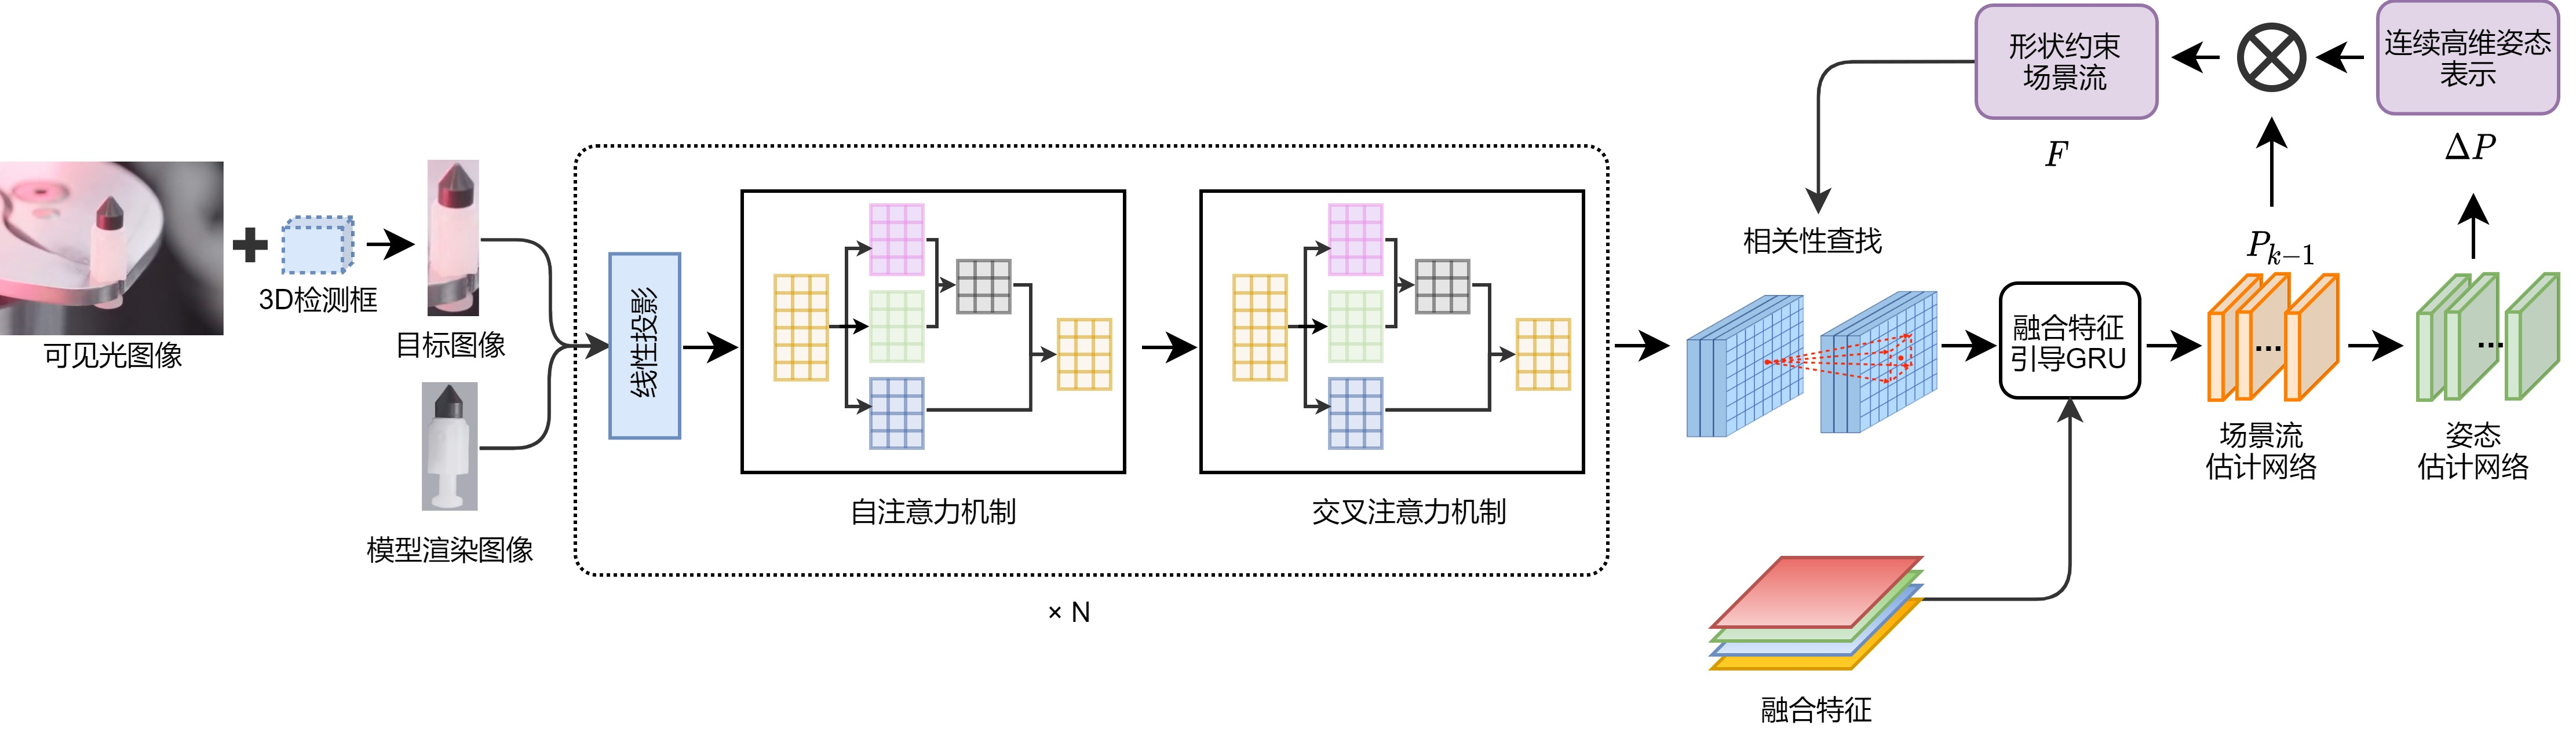
\includegraphics[width=\linewidth]{geo_guided_6d_refine.jpg}
    \caption{基于几何特征引导的6D姿态修正框架}
    \label{fig:geo_guided_6D_refine}
\end{figure}
% 自注意力机制和交叉注意力机制
% 提取-匹配范式
经3D检测算法输出的目标图像和模型在初始位姿下的渲染图像首先进入注意力机制模块。在这一模块中,我们将研究如何利用视觉注意力机制强大的特征提取能力和灵活的特征建模能力来提取得到足够具有表达性的特征。注意力机制是为后续光流估计服务的,但本课题场景与常规光流估计有所不同。一方面,常规光流估计算法依赖图像的浅层特征进行匹配,然而在本课题场景中,网络需要更强的特征提取能力来提取到物体无关的特征,为后续的匹配过程服务。另一方面,常规方案中使用的编码器较为简单,提取出的特征表达性较弱,这导致匹配过程的效率较低,需依赖于多次迭代来进行优化,网络的运行速度较慢。

本方案将结合自注意力机制和交叉注意力机制,如图~\ref{fig:geo_guided_6D_refine}中的中间虚线框所示。
自注意力机制中,对于输入的特征分别进行线性投影,得到$Q$,$K$和$V$,通过计算每个位置的特征与其他位置特征的相似度来调整该位置的特征表示,以此实现特征增强。
交叉注意力机制中,输入为两幅图像的特征$X_1$和$X_2$,对$X_1$进行投影得到$Q$,对于$X_2$进行投影得到$K$和$V$,利用两张图像的相似性来加强它们之间的特征表示,从而实现后续更好的匹配。
这种基于注意力机制的特征增强方式不仅可以提高特征的表达能力,还可以在匹配过程中降低噪声干扰和错误匹配的概率,进一步提高了匹配的精度和鲁棒性。

% 相关性查找
完成注意力机制的特征增强后,我们将通过姿态引导光流进行相关性查找。光流估计网络得到的光流无法反映物体的形状,有很严重的畸变。本课题我们将研究能够通过严格反映物体形状的光流来进行相关性查找的方法,在训练过程中使网络感知到物体的3D几何形状。给定渲染图像的姿态以及当前估计的6D姿态,我们将尝试通过几何计算得到初始渲染图像中的每个像素在当前估计6D姿态下的对应点,这些对应点能够严格反映物体的形状。同时,这种全局感知的方式将能够修正一些不可靠的光流估计,进而得到与全局姿态相符合的对应点,使得这些像素迅速逃离局部解,缩小匹配时的搜索空间。

% 相关性查找
% 残差光流估计的核心操作是通过相关性查找在4D相关体中在当前估计的2D密集匹配以及其周围邻域中进行索引,进而确定在当前估计的2D密集匹配下的相关性。建立在深度特征的连续性假设上,通过在当前估计的光流基础上估计一个偏移,使得估计对应点朝着相关性更高的方向移动,估计的对应点更可能找到目标对应点。本方案考虑引入GRU模块,GRU在序列任务建模中发挥着良好的作用,通过引入门控机制,选择性地保留或者舍弃先前的状态信息。方案研究中,我们将相关性查找得到的相关性特征进一步输入GRU中,更新GRU内部的隐状态,进而利用GRU更新后的隐状态来进行残差光流的预测。


% 融合特征引导GRU
相关性查找后输出的特征将与前级输入的融合特征进行拼接,并将拼接后的特征输入到GRU进行状态的更新。相较于传统的单一特征,融合特征能够提供更丰富全面的信息,从而更好地描述当前的物体,改善GRU的隐状态表示,为后续的场景流回归与姿态回归模型提供支持。GRU的迭代方式可以表示为
\begin{gather}
        z_t = \sigma(\mathrm{Conv}_{3\times3}([h_{t-1}, x_t], W_z)) \\
        r_t = \sigma(\mathrm{Conv}_{3\times3}([h_{t-1}, x_t], W_r)) \\
        \hat{h}_t = \mathrm{tanh}(\mathrm{Conv}_{3\times3}([r_t \otimes h_{t-1}, x_t], W_h)) \\
        h_t = (1 - z_t)\otimes h_{t-1} + z_t \otimes \hat{h}_t
\end{gather}
其中$h_t$即为更新后的隐状态,用来进行后续的场景流回归,$x_t$为相关性特征与融合特征的拼接。
GRU使用三个子网络分别建模遗忘信息的程度$z_t$、更新信息的程度$r_t$以及当前时刻的状态信息$\hat{h}_t$。
通过这三个子网络的交互,GRU可以有效地对迭代更新任务进行建模。

% 形状约束场景流
对于融合特征引导GRU之后的特征图,我们将研究基于场景流的6D姿态修正框架。现有的方案大都使用光流进行相对姿态的回归,忽略了深度变化这一分量,仅从二维层面进行三维特征的回归。尽管可以通过数据驱动的学习方式隐式地将二维光流映射到三维空间,但这是病态的,不利于网络的学习。场景流与光流有所区别,光流估计平面的二维运动,即估计源图像中每个像素在目标图像中的2D对应点。而场景流估计物体的三维运动,即估计源RGB-D图像中每个像素在目标图像中的3D对应点。本方案将尝试基于场景流的几何特征引导框架。在每次迭代中,网络回归残差场景流与残差姿态,将三维场景流进行投影到二维平面,得到形状约束的光流,利用目前成熟的二维相关性查找操作来为残差场景流的估计服务。
更具体地,由于我们使用渲染技术合成初始姿态下的目标物体,相应的深度图$D$是可以得到的,因此可以通过几何推理的方式得到源图像中姿态$P_0$的物体到预测姿态$\hat{P}$下物体的场景流。对于渲染图像中的一个像素$(u_1,v_1)$以及其相应的深度$d_1$,在已知渲染姿态以及相机内参的情况下,利用针孔相机模型反投影函数$\pi^{-1}$将其反投影到物体的CAD模型中,得到其对应的3D点$p=(x,y,z)$,并将点$p$在预测姿态$\hat{P}$下进行投影即可得到其在$\hat{p}$下的对应点$(u_2,v_2)$及其相应的深度$d_2$。
上述过程可以被表述为
\begin{equation}
    (u_2,v_2,d_2) = \pi(\pi^{-1}(u_1, v_1,d_1, k, P_0), k, \hat{p})
\end{equation}
其中$\pi$为针孔相机投影模型,即$d[u~v~1]^T=K(Rp+t)$。因此,场景流可以被表示为$\Delta u = u_2 - u_1, \Delta v = v_2 - v_1, \Delta d = d_2 - d_1$。
该场景流同样能够严格地反映物体的形状,进而将三维几何约束引入匹配过程,减小匹配时的搜索空间。

% 姿态与场景流联合估计
对于图~\ref{fig:geo_guided_6D_refine}姿态修正研究框架中的最后一部分,我们仍将使用经典的四元数作为旋转表示,并采用DeepIM\cite{li2018deepim}中提出的分离相对姿态表示。在联合优化光流和姿态时,优化姿态时的梯度反向传播对光流的优化也有益处。进一步修正光流可以提高姿态估计的精度,因此,良好的姿态表示在我们的框架中至关重要。
相对姿态的表示对网络的学习比绝对姿态有更高的要求,不合理的姿态表示会在网络的优化过程中引入不必要的困难。其中最重要的问题是坐标系的选取。DeepIM提出使用相机下物体的中心作为坐标系的中心,并使用与相机系的坐标轴平行的轴作为坐标系的中心,具体表示为
\begin{equation}
    \begin{aligned}
    \Delta x & = f_x(t_x^{i+1}/t_z^{i+1} - t_x^i/t_z^i)\\
    \Delta y & = f_y(t_y^{i+1}/t_z^{i+1} - t_y^i/t_z^i) \\
    \Delta z & = log(t_z^i/t_z^{i+1})
    \label{eq:relative_pose}
\end{aligned}
\end{equation}
其中,$f_x$与$f_y$为相机的焦距。在这种表示下,$v_x$与$v_y$被定义在图像平面上的位移,而$v_z$被定义为相对尺度的变化,网络可以从两张图像中物体的相对位置与大小推理得到,旋转和平移得以解耦,适合网络的优化。然而,四元数旋转表示在欧几里得空间中是不连续的,不利于神经网络的回归。本课题研究中将尝试将相对三维旋转映射到高维空间,以得到一个连续的相对旋转表示。连续的目标函数可以提供更加稳定的梯度,进而加快相对姿态优化的收敛。

% 可行性分析
本部分的位姿修正方案,申请人团队已在基于光流的算法框架中初步验证了可行性。实验过程中,我们首先利用目前成熟的 6D 姿态估计网络预测得到一个不精确的初始6D 姿态$P_0$,之后利用该姿态对目标进行渲染和定位。对于输入的一张目标RGB图像和在初始姿态$P_0$下渲染的目标模型图像,实验方案首先利用一个孪生卷积神经网络来对该两张图像进行特征提取,分别得到维度为$H\times W$的特征图$g_1$和$g_2$。之后根据提取的特征向量构建4D相关体$C$,$C$的维度为$H\times W \times H \times W$,其中    $C_{ijkl} = g^1_{ij} \cdot g^2_{kl}$,
$C$表示了$g_1$中所有特征向量与$g_2$中所有特征向量的相关性。
然后,实验过程中,在每次迭代中同时估计残差光流$\Delta F$与残差姿态$\Delta P$,并进行估计姿态的更新,即$P_i = \Delta P_i \otimes P_{i-1}$。其中,我们利用一个单独的姿态估计网络$f_{\theta}$通过估计的残差光流进行残差姿态的回归,即$\Delta P_i = f_{\theta}(\Delta F)$,
$f_\theta$由若干层卷积层与全连接层组成,最终由两个支路分别预测旋转$\Delta R$与平移$\Delta t$。实验结果表明???

上述研究方案中的关键技术问题将通过图\ref{fig:research_solution}所示所示的流程逐步开展研究,通过理论分析和实验验证逐步完善算法,验证方案的性能。


\NsfcSection{4}{本项目的特色与创新之处;}{}

本项目是在我国航天工业生产实践中提出的问题,但问题本身在其他危化品制造行业中普遍存在。由于问题研究的场景有针对性,因此课题研究的方法也有显著特色,对应的创新之处主要有三方面:

1. 危化品制造中的目标物体纹理弱,但通常都包含特殊材质,这类材质在特定光谱谱段有单峰响应,本项目研究如何用多源融合表征技术解决这一问题。通过引入光谱图像与可见光图像交叉注意力融合,弥补可见光图像在危化品零部件细节特征提取上的不足,同时通过深度图像生成的点云特征与可见光图像特征的交叉融合得到补全点云全局特征,弥补可见光图像三维几何信息的缺失。

2. 智能制造场景中目标物体存在遮挡现象,本项目引入刚性感知的检测方法解决姿态估计的鲁棒性问题。研究方案提出一种新颖的基于距离函数的距离变换图,可以取代2D检测的图像掩膜标注以及3D点云的逐点分割掩膜,且可以利用距离变换图指导网络在训练期间仅由目标可见部分的正特征单元监督而不受遮挡部分的干扰。此外,方案引入2D候选引导的3D候选融合策略来对3D检测候选置信度进行处理,并且设计了融合候选局部预测的方法避免非最大抑制方法对正确检测候选的抑制,预期能在遮挡情况下取得更准确的检测结果。

3. 在弱纹理目标无法有效引导姿态修正的情况下,本项目研究如何通过几何特征引导6D姿态修正,计算高精度的位姿估计结果。项目将通过可微相对姿态求解层逐步优化6D位姿,并将几何信息引入特征匹配过程,使得匹配得到的特征与物体的几何形状一致。同时,将显式地使用深度神经网络编码几何特征作为姿态修正网络的参考信息,提升姿态估计的最终精度,为智能抓取提供可靠输入。

\NsfcSection{5}{年度研究计划及预期研究结果}{(包括拟组织的重要学术交流活动、国际合作与交流计划等)。}

\subsection{年度研究计划}

本课题研究期限从2024年1月到2027年12月。年度计划如下:  

2024.01-2024.06,基于公开的RGB-D目标6D姿态估计数据集,人工标记模拟光谱图,构建实验数据集,支撑项目前期研究工作。同时,在合作研究所的产线上布置真实实验环境。选定特定危化品类型,通过实验获得最佳光谱谱段。将智能装配车间的可见光相机位置,增加深度相机和光谱相机。捕获装配目标场景下的深度图像和光谱图像。完成可见光影像、深度图和光谱影像之间的配准,并清洗数据,构建完整可用的多模态融合数据集。拟发表国际期刊论文1\textasciitilde2篇,形成的数据集对学术界开放下载。

2024.07-2025.02,可见光图像特征提取网络中的特征通道注意力机制研究。分析和研究$N\times N$卷积模块的卷积核大小和深度对特征提取结果的影响,结合现有的后端姿态估计网络,验证灵活卷积核的配置方式,拟发表国际期刊论文1\textasciitilde2篇,其中包括一篇国际顶会论文,参加CVPR或ECCV国际会议与同行交流。

2025.03-2025.8,交叉融合注意力机制中的点云特征补全方法研究。通过研究点云特征与可见光图像特征的空间映射关系,分析交叉融合注意力图生成机制,引导可见光图像特征融合点云特征,解决点云三维空间特征缺失的问题。拟发表国际期刊论文1\textasciitilde2篇,其中包括一篇国际顶会论文,参加CSIG的3DV专委会年度会议,与同行交流。

2025.09-2025.12,多模态特征融合机制研究。研究光谱特征和可见光图像特征交叉融合机制,引导光谱特征增强可见光图像特征的表征能力,解决可见光图像细节特征不完整的问题。拟发表国际期刊论文1\textasciitilde2篇,其中包括一篇国际顶会论文,参加国际会议与同行交流。多源融合表征方面的代码成果整理发布,供同行参考讨论。

2026.01-2026.06,复杂环境下的 3D 目标检测网络研究。以多模态数据及其融合数据作为模型的输入,研究基于刚性感知、关键点定位及候选预测融合的 3D 目标检测框架,为后续高精度的姿态估计提供精准的空间信息。拟发表国际期刊论文1\textasciitilde2篇,其中包括一篇国际顶会论文。与CCF-CV专委会中自动驾驶方面的学者交流类似方法的改进策略。

2026.07-2027.03,基于工件几何特征引导的位姿修正方法研究。拟发表国际期刊论文1\textasciitilde2篇,其中包括一篇国际顶会论文,参加国际会议与同行交流。就几何特征引导的位姿修正问题与Mathieu教授安排一次专题学术会议,并邀请相关学者研讨。

2027.04-2027.12,在真实智能装配场景下完成算法适应性实验,分析精度误差来源,进一步改进位姿修正方法,提升算法在真实场景下的精度和鲁棒性。拟发表国际期刊论文1\textasciitilde2篇,其中包括一篇国际顶会论文,参加国际会议与同行交流。

\subsection{预期研究成果}

本项目预期发表学术研究论文10篇,其中顶会或顶刊论文8篇,申请专利和软件著作权8件,在三个关键研究内容方面的算法成果将在github上对外发布代码,相应的实验数据集也将一并发布。本项目的研究有很强的应用背景,研究内容之间模块化和体系化较强,研究成果也将指导真实装配流程,实际运行的结果将在国际会议上进行成果展示。研究期间将培养博士研究生3\textasciitilde4名,硕士研究生12\textasciitilde15名。

%%%%%%%%%%%%%%%%%%%%%%%%%%%%%%%%%%%%%%%%%%%%%%%%%
\ContentDes{(二)研究基础与工作条件}

\NsfcSection{1}{研究基础}{
(与本项目相关的研究工作积累和已取得的研究工作成绩);}

\subsection{工作基础}


本课题的研究不仅需要位姿估计方面的基础,对于光谱特征提取、目标检测和光流估计也需有较为深入的理解。申请人课题组在这几个方面都有深入的研究。
\myPara{位姿估计方面}
申请人团队与Magic Leap的Yinlin Hu博士,以及EPFL的Mathieu教授保持长期合作。Yinlin Hu为申请人指导的博士生,于2018年推荐到EFPL做博士后研究。在前期合作研究中联合指导课题组的博士和硕士研究生。团队在2022年10月参加了ECCV的BOP 6D姿态挑战赛,并在Single-Model赛道获得冠军。2023年团队有两篇IEEE国际顶会CVPR论文被录用,其中一篇为“\#2298 Yang Hai, Rui Song, Jiaojiao Li, Mathieu Salzmann, Yinlin Hu. Rigidity-Aware Detection for 6D Object Pose Estimation. IEEE CVPR2023 ”,另一篇为“\#2307 Yang Hai, Rui Song, Jiaojiao Li, Yinlin Hu. Shape-Constraint Recurrent Flow for 6D Object Pose Estimation. IEEE CVPR2023”。

\iffalse
\subsection{---SR修改分割线---}
\fi
\myPara{光流估计方面}
申请人团队在光流估计方面有相关技术积累,并在6D姿态估计算法中集成了光流估计的计算流程。申请人曾在CVPR发表两篇论文,一篇为Hu, Yinlin and Song, Rui and Li, Yunsong., “Efficient Coarse-to-Fine Patch Match for Large Displacement Optical Flow,” in 2016 IEEE Conference on Computer Vision and Pattern Recognition (CVPR), Jun. 2016, pp. 5704–5712.该论文为Spotlight,解决大位移情况下的光流估计问题。另一篇为Hu, Yinlin and Li, Yunsong and Song, Rui, “Robust Interpolation of Correspondences for Large Displacement Optical Flow”, in 2017 IEEE Conference on Computer Vision and Pattern Recognition (CVPR), Jul. 2017, no. July, pp. 4791–4799.解决稠密光流中的鲁棒插值问题。此外,申请人太对发表在Image and Vision Computing上的论文Hu, Yinlin and Song, Rui and Li, Yunsong and Rao, Peng and Wang, Yangli, “Highly accurate optical flow estimation on superpixel tree,” Image Vis. Comput., vol. 52, pp. 167–177, Aug. 2016.已被OpenCV收录。上述三篇论文的代码均已在github开源。

\myPara{深度图的点云处理方面}
申请人团队在点云分类、语义分割、点云补全等点云处理主流任务上都进行了相关研究,在领域国际顶会与核心期刊上发表了四篇论文。其中一篇为“Fengda Hao, Jiaojiao Li*, Rui Song*, Yunsong Li and Kailang Cao. Structure-Aware Graph Convolution Network for Point Cloud Parsing.”发表在计算机视觉领域中科院一区期刊IEEE Transactions on Multimedia上;一篇为“Fengda Hao, Rui Song*, JiaoJiao Li*, Kailang Cao, Yunsong Li. Cascaded Geometric Feature Modulation Network for Point Cloud Processing.”发表在计算机学科国际学术期刊Neurocomputing上,一篇为“Fengda Hao, Jiaojiao Li, Rui Song, Yunsong Li and Kailang Cao. Mixed Feature Prediction on Boundary Learning for Point Cloud Semantic Segmentation.”发表在遥感领域权威期刊Remote Sensing上。另外,申请人团队2021年在国际计算机多媒体领域顶级会议ACM Multimedia 2021上发表题为“ASFM-Net: Asymmetrical Siamese Feature Matching Network for Point Completion”的研究成果。该项成果在2021年斯坦福大学发布的Completion3D点云补全任务榜单中排列第一。

\myPara{光谱图像目标检测方面}
光谱目标检测也是申请人团队的研究内容之一,团队成员在2022年在相关领域国际高水平期刊上发表了多篇SCI论文,代表性论文有“J. Li, H. Zhang, R. Song, W. Xie, Y. Li and Q. Du, Structure-Guided Feature Transform Hybrid Residual Network for Remote Sensing Object Detection.”发表在遥感领域中科院一区TOP期刊IEEE Transactions on Geoscience and Remote Sensing上,该工作提出了一种新的结构引导的特征变换混合残差(SGFTHR)网络,可以以无锚的方式克服在不同尺度上目标检测的低性能,尤其是对于小而密集的目标,提升了检测性能。

\myPara{多源融合方面}
在多源融合方面,申请人在遥感图像处理领域中科院一区TOP期刊IEEE Transactions on Geoscience and Remote Sensing上发表了多篇相关论文,其中一篇为J. Li, Y. Liu, R. Song, Y. Li, K. Han, and Q. Du, “Sal2RN: A Spatial-Spectral Salient Reinforcement Network for Hyperspectral and LiDAR Data Fusion Classification,” IEEE Trans. Geosci. Remote Sens., vol. 14, no. 8, pp. 1–1, 2022,论文提出了基于跨层特征提取和互补融合策略的深度学习网络,用于LiDAR和Hyperspectral联合分类,提升了LiDAR和Hyperspectral的分类性能;一篇为J. Li, Y. Ma, R. Song, B. Xi, D. Hong, and Q. Du, “A Triplet Semisupervised Deep Network for Fusion Classification of Hyperspectral and LiDAR Data,” IEEE Trans. Geosci. Remote Sens., vol. 60, pp. 1–13, 2022,提出了一种级联神经网络来提取LiDAR深度特征,提升了LiDAR和Hyperspectral图像的融合感知性能;一篇为Y. Li, Y. Zheng, J. Li, R. Song, and J. Chanussot, “Hyperspectral Pansharpening With Adaptive Feature Modulation-Based Detail Injection Network,” IEEE Trans. Geosci. Remote Sens., vol. 60, 2022,提出一种基于自适应特征调制的细节注入融合网络,提升PAN和Hyperspectral的融合性能。

\subsection{研究工作获奖}

\myPara{ECCV2022 BOP 6D姿态估计挑战赛单模型赛道冠军}
申请人团队在计算机视觉顶级会议ECCV 2022举办的BOP 6D位姿估计挑战赛中获得了最佳单模型奖项“The Best Single-Model Method”(链接地址\url{https://cmp.felk.cvut.cz/sixd/workshop_2022/slides/bop_challenge_2022_results.pdf}),竞赛中提出的方法可以同时处理单目RGB以及RGB-D图像,可扩展性较强。

\myPara{2019年中央军委“天智杯”人工智能挑战赛冠军}
申请人团队2019年12月19日参加了由军委装备发展部指导,航天系统部主办的我国首届“天智杯”人工智能挑战赛。挑战赛题目是以主办方提供的光学卫星遥感影像为处理对象,难点为全色影像与RGB影像同时存在,且在大场景范围影像中同时完成四类典型地物要素的像素级分割,获得地物要素精确轮廓边缘和属性信息,申请人团队针对数据特点,创新性提出了空间-通道最大化注意力机制为核心的网络模型,并使用了决策级融合和特征级融合的策略,最终得到了精确且鲁棒性的分割结果,在科目二竞赛中获得第一名。

\NsfcSection{2}{工作条件}{
(包括已具备的实验条件,尚缺少的实验条件和拟解决的途径,包括利用国家实验室、国家重点实验室和部门重点实验室等研究基地的计划与落实情况);}

本项目在数据采集和数据集制作中,需要具备可见光相机、深度相机和光谱相机等核心硬件设备。在真实场景验证中,需要有目标工件和机械臂等辅助设备。算法研究和验证方面需要深度学习服务器。研究工作需团队成员协作。基于申请人团队已有的工作基础,具备上述条件即可开展项目的研究工作。

申请人团队率属于综合业务网理论及关键技术国家重点实验室,实验室有完备的科研场地和专业设备。已具备的实验条件包括:
\begin{itemize}
    \item 高分辨率可见光相机。最高空间分辨率5K×4K,可输出原始图像数据。
    \item ZED深度相机。工作距离0.2\textasciitilde20m,空间分辨率1920×1080。
    \item Headwall高光谱成像光谱仪Micro-Hyperspec SWIR M640。光谱覆盖范围400nm\textasciitilde2500nm,能够满足本项目对危化品样品拍摄时的光谱实验要求。
    \item 光学散射片、红外片、反射镜、棱镜、成像靶标等辅助设备,这些设备在真实场景拍摄情况下能为特定光谱数据的采集提供支撑。
    \item 高精度激光三维扫描仪。加拿大Creaform3D/GoScan Spark,对给定的无纹理工件,通过扫描获得高精度的三维模型,模型精度50μm,能够支撑本项目基于模型引导的位姿优化部分的研究。
    \item 深度学习服务器。专业深度学习服务器,配额支持10卡3090,能够满足本项目深度学习算法训练和调试的需要。
\end{itemize}
此外,申请人团队已与西安航天自动化股份有限公司(航天科工集团六院下属)成立了秦创原科学家+工程师团队,公示网址\url{https://kjt.shaanxi.gov.cn/kjzx/tzgg/296970.html}。该公司可为本项目的研究提供装配试验场地、目标工件和机械臂等自动化设备。

目前尚缺少的实验条件及拟解决途径包括
\begin{itemize}
    \item 用于多源融合算法设计的特殊材质耗材。本项目执行过程中,为了使数据多样化,满足网络训练的需要,将购置一部分特殊材质的目标工件,通过3D扫描获得工件的三维模型。
    \item 光谱相机镀膜。目前实验室设备为专用高光谱设备,谱段覆盖范围宽,但设备尺寸大,不适合于特定光谱数据的高速采集。本项目执行过程中将委托中国科学院上海技术物理研究所或8358所定制镀膜,将现有相机改造为特定光谱相机。
    \item 多源图像采集系统的集成。目前可见光相机、深度相机和光谱相机仍为分立设备,本项目执行过程中需定制支架、线缆等,对设备环境进行改造。使改造后的设备能对同一场景同时输出可见光图、深度图和光谱图。
\end{itemize}



\myPara{经费和硬件条件方面}我们


\myPara{人员方面}我们

\myPara{国内外合作方面} 我们


\NsfcSection{3}{正在承担的与本项目相关的科研项目情况}{
(申请人和主要参与者正在承担的与本项目相关的科研项目情况,包括国家自然科学基金的项目和国家其他科技计划项目,要注明项目的资助机构、项目类别、批准号、项目名称、获资助金额、起止年月、与本项目的关系及负责的内容等);}

已获批一项陕西省重点研发计划“科学家+工程师”队伍建设项目,项目名称为《航天装备智能制造“科学家+工程师”队伍》,公示链接\url{https://kjt.shaanxi.gov.cn/kjzx/tzgg/296970.html},项目资助总金额为30万元,起止年月为2023年1月至2025年12月。该项目为申请人团队与西安航天自动化股份有限公司联合申报的团队建设项目,主要经费用于企业硬件平台的搭建。西安航天自动化股份有限公司是我国航天特种装备的主要生产企业,在该项目的支持下,申请人团队将在企业产线上搭建一套完整的多模态融合采集硬件平台,为本项目的顺利执行打好基础。本项目研发的成果,也将应用于合作企业的实际智能装备生产流程中,为我国的智能制造装备升级提供理论支撑。


\NsfcSection{4}{完成国家自然科学基金项目情况}{
(对申请人负责的前一个已资助期满的科学基金项目(项目名称及批准号)完成情况、后续研究进展及与本申请项目的关系加以详细说明。另附该项目的研究工作总结摘要(限500字)和相关成果详细目录)。}

补充中...

%%%%%%%%%%%%%%%%%%%%%%%%%%%%%%%%%%%%%%%%%%%%%%%%%
\ContentDes{(三) 其他需要说明的问题}



\NsfcSection{1}{}{
申请人同年申请不同类型的国家自然科学基金项目情况(列明同年申请的其他项目的项目类型、项目名称信息,并说明与本项目之间的区别与联系)。}

同年参与另外一项自然科学基金面上项目的申请,项目类型为面上项目,项目名称为...

该项目与本项目的侧重点不同。

\NsfcSection{2}{}{
具有高级专业技术职务(职称)的申请人或者主要参与者是否存在同年申请或者参与申请国家自然科学基金项目的单位不一致的情况;如存在上述情况,列明所涉及人员的姓名,申请或参与申请的其他项目的项目类型、项目名称、单位名称、上述人员在该项目中是申请人还是参与者,并说明单位不一致原因。}

无。

\NsfcSection{3}{}{
具有高级专业技术职务(职称)的申请人或者主要参与者是否存在与正在承担的国家自然科学基金项目的单位不一致的情况;如存在上述情况,列明所涉及人员的姓名,正在承担项目的批准号、项目类型、项目名称、单位名称、起止年月,并说明单位不一致原因。}

无。

\NsfcSection{4}{}{其他。}

无。


\end{document}
